\PassOptionsToPackage{unicode=true}{hyperref} % options for packages loaded elsewhere
\PassOptionsToPackage{hyphens}{url}
%
\documentclass[]{article}
\usepackage{lmodern}
\usepackage{amssymb,amsmath}
\usepackage{ifxetex,ifluatex}
\usepackage{fixltx2e} % provides \textsubscript
\ifnum 0\ifxetex 1\fi\ifluatex 1\fi=0 % if pdftex
  \usepackage[T1]{fontenc}
  \usepackage[utf8]{inputenc}
  \usepackage{textcomp} % provides euro and other symbols
\else % if luatex or xelatex
  \usepackage{unicode-math}
  \defaultfontfeatures{Ligatures=TeX,Scale=MatchLowercase}
\fi
% use upquote if available, for straight quotes in verbatim environments
\IfFileExists{upquote.sty}{\usepackage{upquote}}{}
% use microtype if available
\IfFileExists{microtype.sty}{%
\usepackage[]{microtype}
\UseMicrotypeSet[protrusion]{basicmath} % disable protrusion for tt fonts
}{}
\IfFileExists{parskip.sty}{%
\usepackage{parskip}
}{% else
\setlength{\parindent}{0pt}
\setlength{\parskip}{6pt plus 2pt minus 1pt}
}
\usepackage{hyperref}
\hypersetup{
            pdfborder={0 0 0},
            breaklinks=true}
\urlstyle{same}  % don't use monospace font for urls
\usepackage{color}
\usepackage{fancyvrb}
\newcommand{\VerbBar}{|}
\newcommand{\VERB}{\Verb[commandchars=\\\{\}]}
\DefineVerbatimEnvironment{Highlighting}{Verbatim}{commandchars=\\\{\}}
% Add ',fontsize=\small' for more characters per line
\newenvironment{Shaded}{}{}
\newcommand{\AlertTok}[1]{\textcolor[rgb]{1.00,0.00,0.00}{\textbf{#1}}}
\newcommand{\AnnotationTok}[1]{\textcolor[rgb]{0.38,0.63,0.69}{\textbf{\textit{#1}}}}
\newcommand{\AttributeTok}[1]{\textcolor[rgb]{0.49,0.56,0.16}{#1}}
\newcommand{\BaseNTok}[1]{\textcolor[rgb]{0.25,0.63,0.44}{#1}}
\newcommand{\BuiltInTok}[1]{#1}
\newcommand{\CharTok}[1]{\textcolor[rgb]{0.25,0.44,0.63}{#1}}
\newcommand{\CommentTok}[1]{\textcolor[rgb]{0.38,0.63,0.69}{\textit{#1}}}
\newcommand{\CommentVarTok}[1]{\textcolor[rgb]{0.38,0.63,0.69}{\textbf{\textit{#1}}}}
\newcommand{\ConstantTok}[1]{\textcolor[rgb]{0.53,0.00,0.00}{#1}}
\newcommand{\ControlFlowTok}[1]{\textcolor[rgb]{0.00,0.44,0.13}{\textbf{#1}}}
\newcommand{\DataTypeTok}[1]{\textcolor[rgb]{0.56,0.13,0.00}{#1}}
\newcommand{\DecValTok}[1]{\textcolor[rgb]{0.25,0.63,0.44}{#1}}
\newcommand{\DocumentationTok}[1]{\textcolor[rgb]{0.73,0.13,0.13}{\textit{#1}}}
\newcommand{\ErrorTok}[1]{\textcolor[rgb]{1.00,0.00,0.00}{\textbf{#1}}}
\newcommand{\ExtensionTok}[1]{#1}
\newcommand{\FloatTok}[1]{\textcolor[rgb]{0.25,0.63,0.44}{#1}}
\newcommand{\FunctionTok}[1]{\textcolor[rgb]{0.02,0.16,0.49}{#1}}
\newcommand{\ImportTok}[1]{#1}
\newcommand{\InformationTok}[1]{\textcolor[rgb]{0.38,0.63,0.69}{\textbf{\textit{#1}}}}
\newcommand{\KeywordTok}[1]{\textcolor[rgb]{0.00,0.44,0.13}{\textbf{#1}}}
\newcommand{\NormalTok}[1]{#1}
\newcommand{\OperatorTok}[1]{\textcolor[rgb]{0.40,0.40,0.40}{#1}}
\newcommand{\OtherTok}[1]{\textcolor[rgb]{0.00,0.44,0.13}{#1}}
\newcommand{\PreprocessorTok}[1]{\textcolor[rgb]{0.74,0.48,0.00}{#1}}
\newcommand{\RegionMarkerTok}[1]{#1}
\newcommand{\SpecialCharTok}[1]{\textcolor[rgb]{0.25,0.44,0.63}{#1}}
\newcommand{\SpecialStringTok}[1]{\textcolor[rgb]{0.73,0.40,0.53}{#1}}
\newcommand{\StringTok}[1]{\textcolor[rgb]{0.25,0.44,0.63}{#1}}
\newcommand{\VariableTok}[1]{\textcolor[rgb]{0.10,0.09,0.49}{#1}}
\newcommand{\VerbatimStringTok}[1]{\textcolor[rgb]{0.25,0.44,0.63}{#1}}
\newcommand{\WarningTok}[1]{\textcolor[rgb]{0.38,0.63,0.69}{\textbf{\textit{#1}}}}
\usepackage{graphicx,grffile}
\makeatletter
\def\maxwidth{\ifdim\Gin@nat@width>\linewidth\linewidth\else\Gin@nat@width\fi}
\def\maxheight{\ifdim\Gin@nat@height>\textheight\textheight\else\Gin@nat@height\fi}
\makeatother
% Scale images if necessary, so that they will not overflow the page
% margins by default, and it is still possible to overwrite the defaults
% using explicit options in \includegraphics[width, height, ...]{}
\setkeys{Gin}{width=\maxwidth,height=\maxheight,keepaspectratio}
\setlength{\emergencystretch}{3em}  % prevent overfull lines
\providecommand{\tightlist}{%
  \setlength{\itemsep}{0pt}\setlength{\parskip}{0pt}}
\setcounter{secnumdepth}{0}
% Redefines (sub)paragraphs to behave more like sections
\ifx\paragraph\undefined\else
\let\oldparagraph\paragraph
\renewcommand{\paragraph}[1]{\oldparagraph{#1}\mbox{}}
\fi
\ifx\subparagraph\undefined\else
\let\oldsubparagraph\subparagraph
\renewcommand{\subparagraph}[1]{\oldsubparagraph{#1}\mbox{}}
\fi

% set default figure placement to htbp
\makeatletter
\def\fps@figure{htbp}
\makeatother

\usepackage{subcaption}

\date{}

\begin{document}

\hypertarget{haptic-labyrinth-final-project}{%
\section{Haptic Labyrinth -- Final
Project}\label{haptic-labyrinth-final-project}}

\hypertarget{philipp-mildenberger-philipp-pobitzer}{%
\subsubsection{Philipp Mildenberger, Philipp
Pobitzer}\label{philipp-mildenberger-philipp-pobitzer}}

\hypertarget{labyrinth}{%
\subsection{Labyrinth}\label{labyrinth}}

\begin{figure}
\hypertarget{fig:lab}{%
\centering
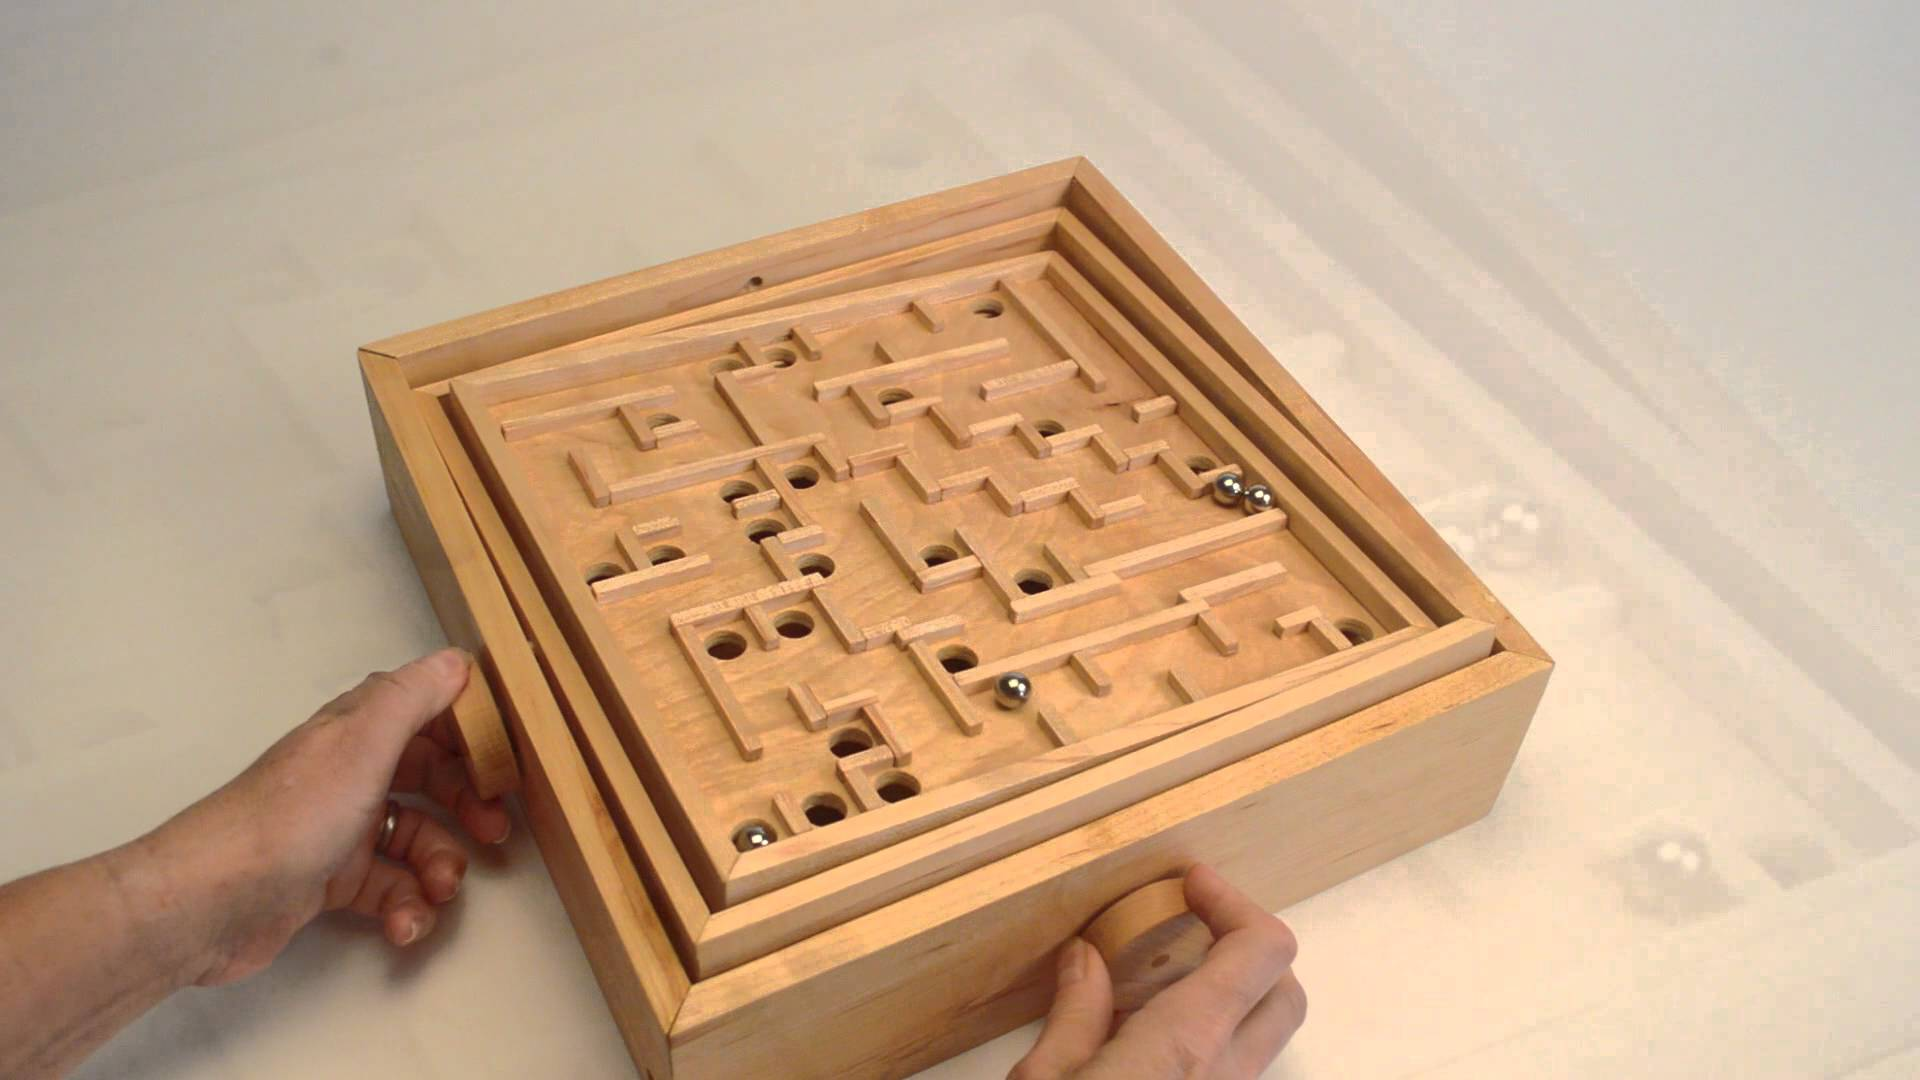
\includegraphics[width=1\textwidth,height=\textheight]{./woodenLabyrinthHands.jpg}
\caption{Labyrinth}\label{fig:lab}
}
\end{figure}

Labyrinth is a classical game consisting of a box with a maze on top
with holes, and a marble. The object of the game is to try to adjust the
play-field to guide the marble out of the maze, without letting it fall
into any of the holes, if there are any. It is controlled via two knobs.
These knobs control a rotation along the two degrees of freedom the
suspended maze has. A wooden version can be seen in Figure
\ref{fig:lab}.

\hypertarget{overview}{%
\subsection{Overview}\label{overview}}

\begin{figure}[h!]
    \begin{subfigure}{0.5\textwidth}
        \centering
        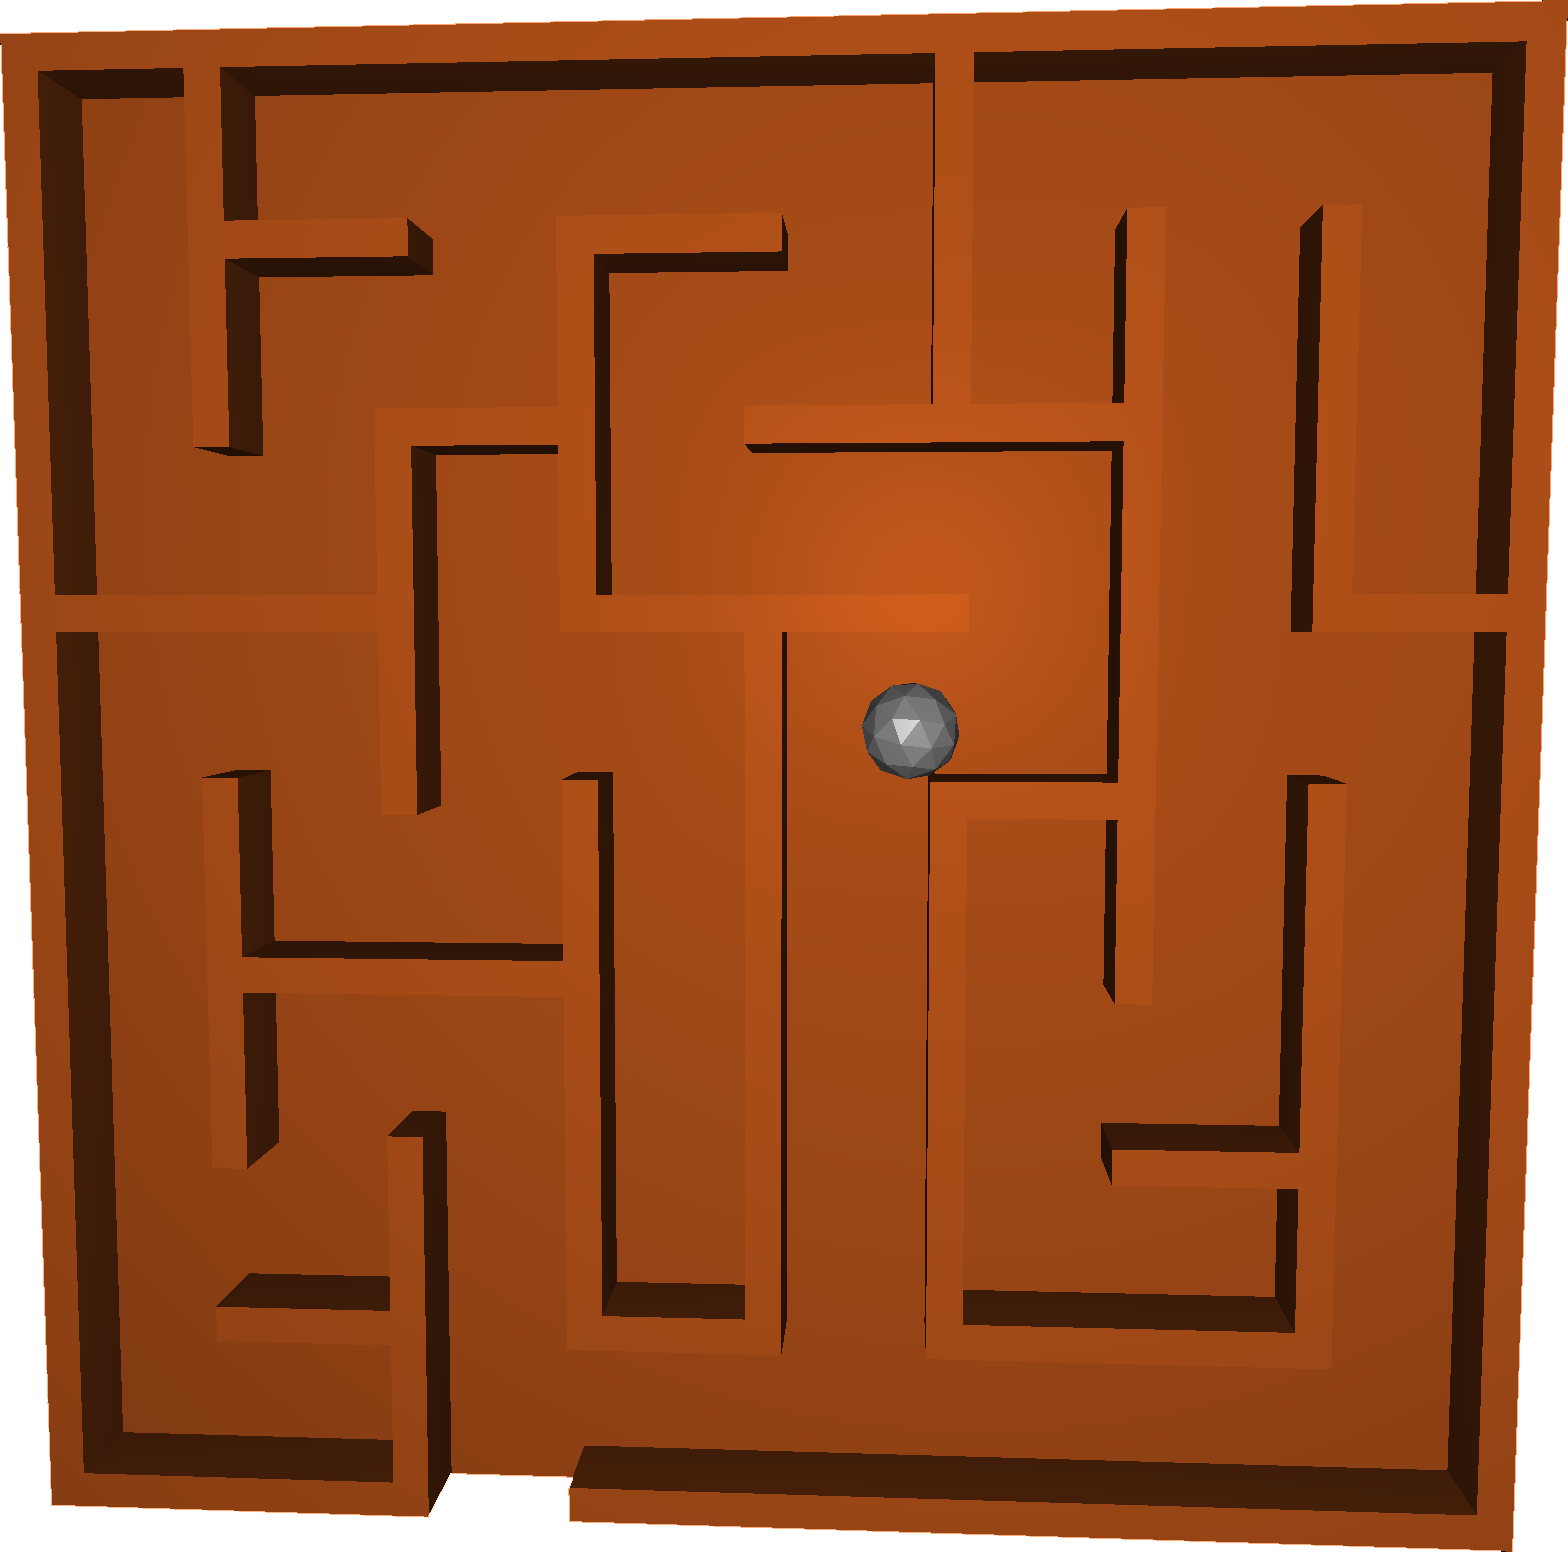
\includegraphics[width=0.8\textwidth]{./labyrinthRender.png}
        \caption*{Render of the application}
    \end{subfigure}%
    \begin{subfigure}{0.5\textwidth}
        \centering
        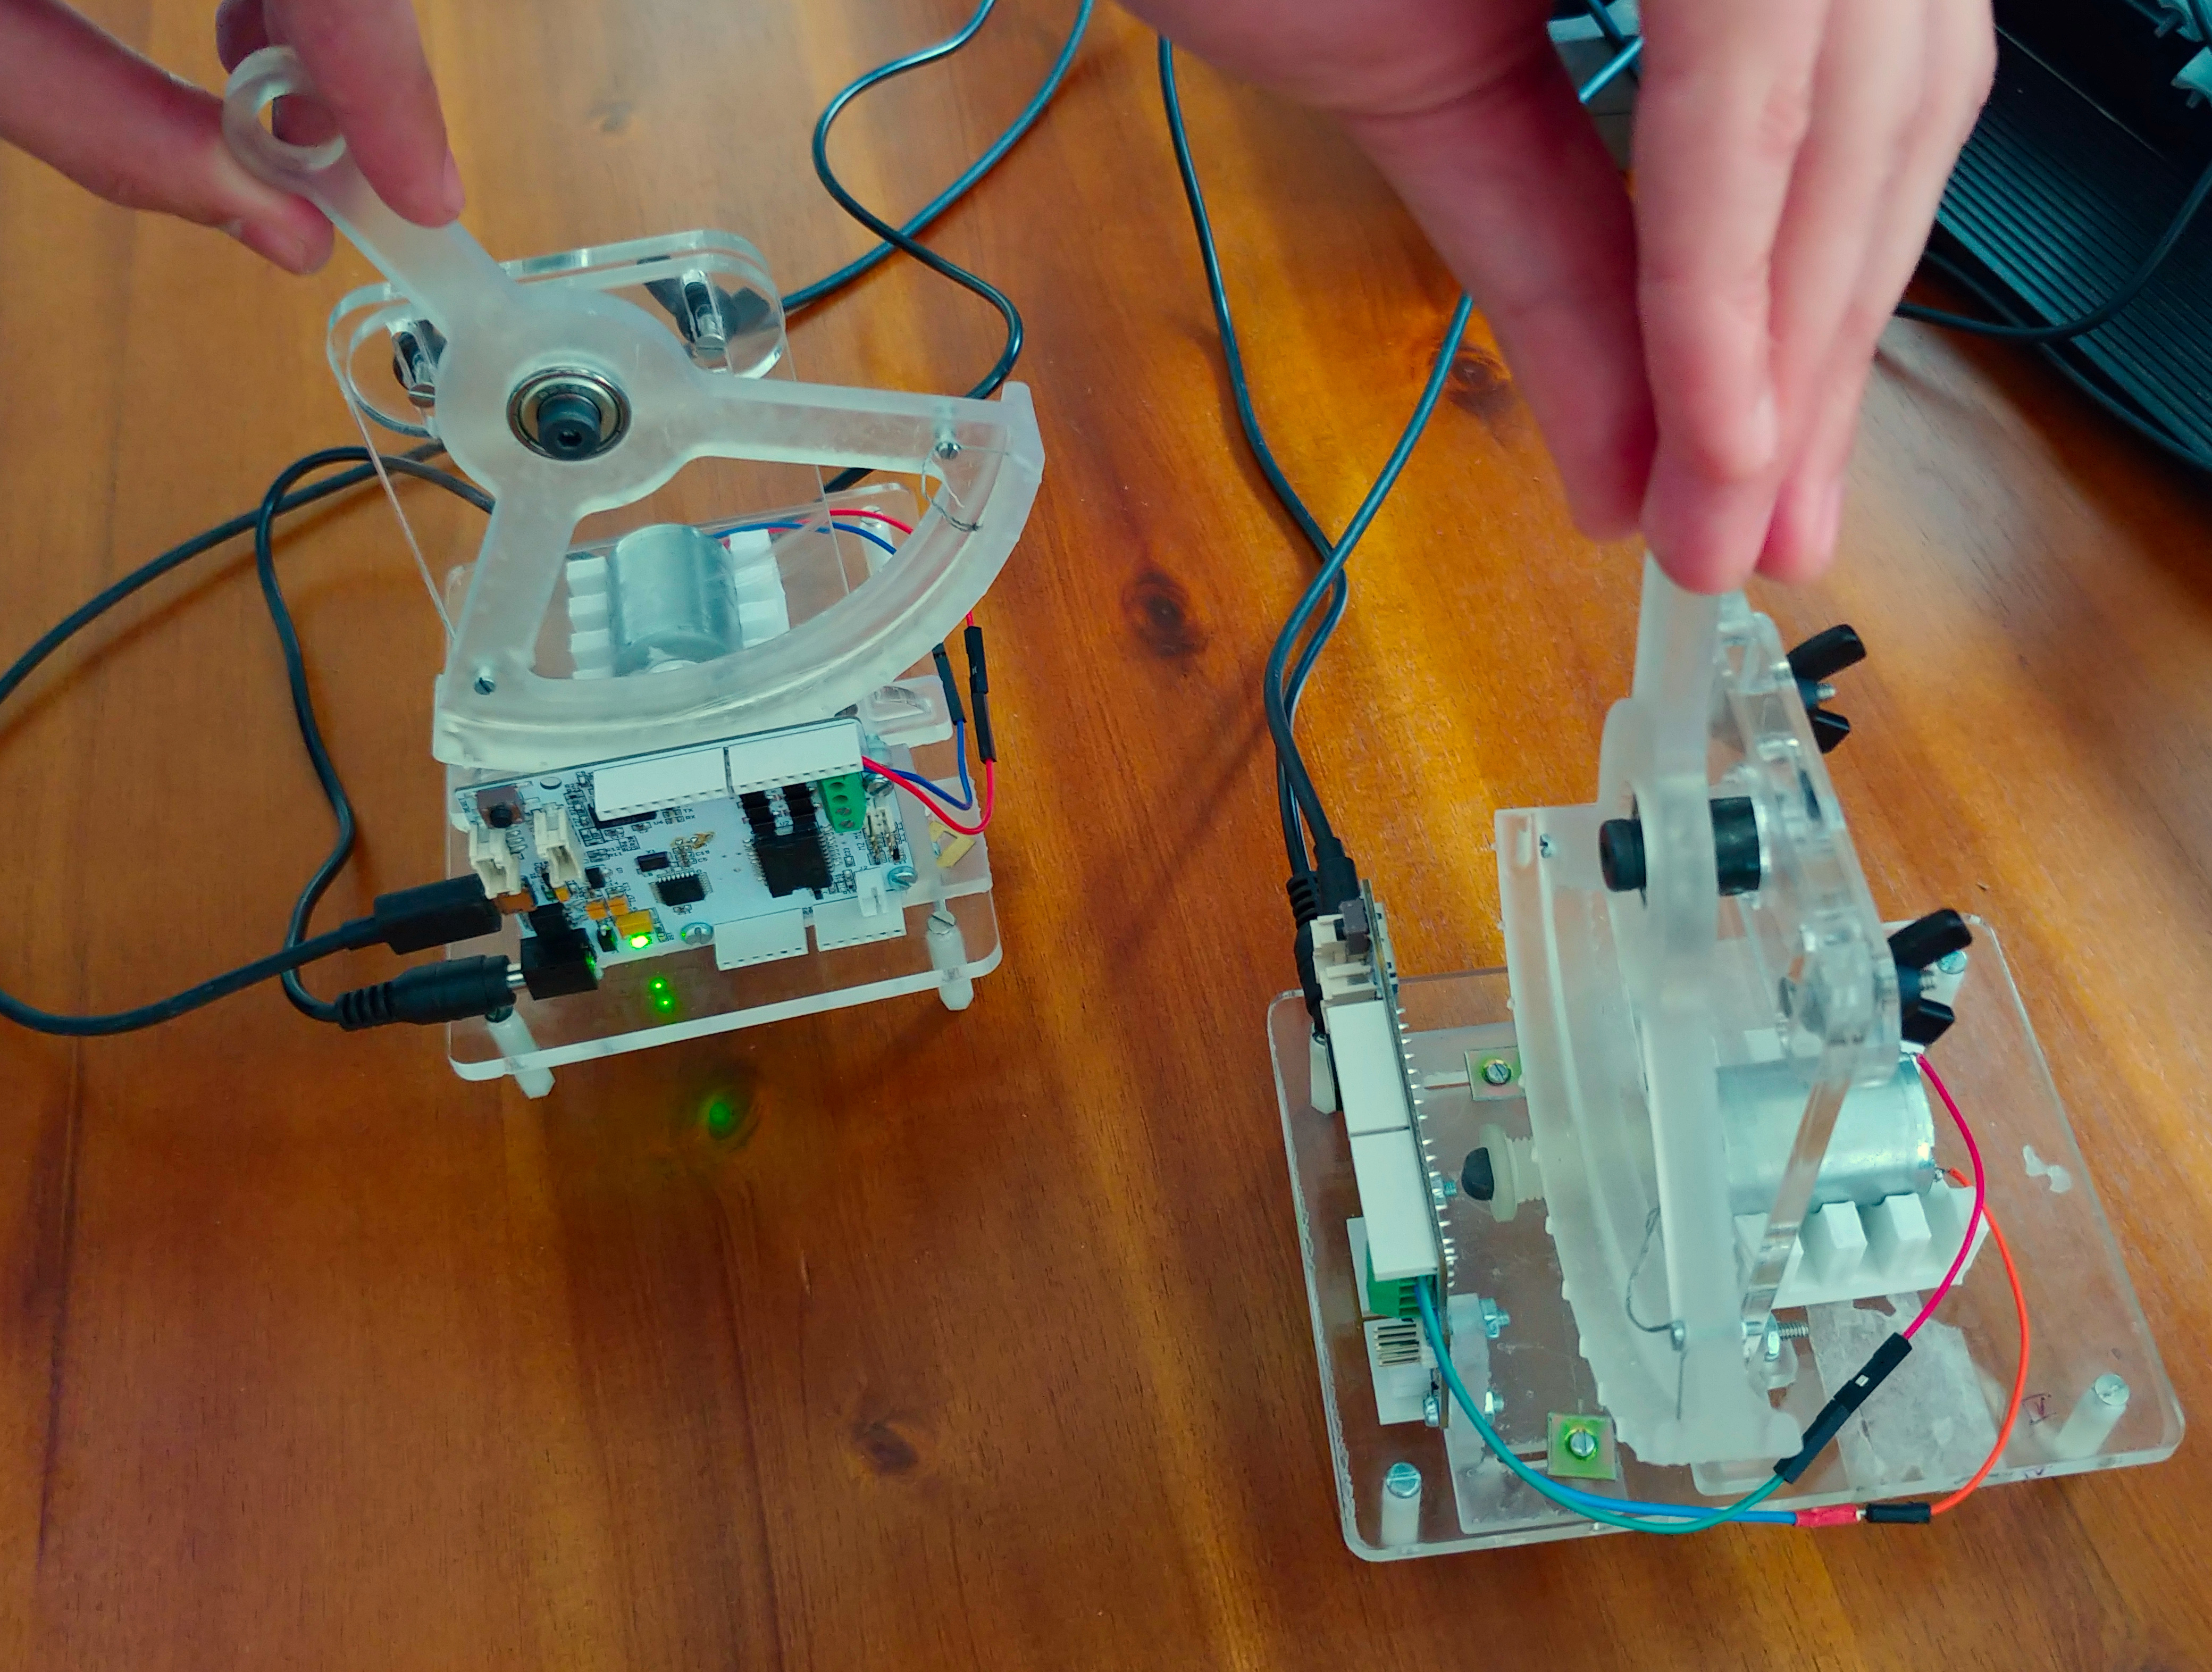
\includegraphics[width=0.8\textwidth]{./hapkitHandles.jpg}
        \caption*{Haptic input controllers}
    \end{subfigure}
    \caption{Application in action}
    \label{fig:app}
\end{figure}

Our colleague Stefan Spiss has implemented a labyrinth as the final
project in physically based simulation. A screenshot of the application
in action can be seen in Figure \ref{fig:app}. We augmented this
application with the possibility to use two Hapkits to control the game.
Each Hapkit models one knob and therefore controls one of the two
degrees of freedom the maze has.

The implementation contains 3 different haptic feedbacks, which are
explained in more detail in the following sections

\hypertarget{virtual-wall}{%
\subsubsection{Virtual Wall}\label{virtual-wall}}

For each handle virtual walls limit the moving range of the handle, it
uses a simulated spring to pull back the handles into defined range,
using the following formula, if the predefined range is exceeded:

\begin{Shaded}
\begin{Highlighting}[]
\NormalTok{    glm::vec2 getWallForce()}
\NormalTok{    \{}
        \KeywordTok{auto}\NormalTok{      pos1 = handleInterface.getPos1();}
        \KeywordTok{auto}\NormalTok{      pos2 = handleInterface.getPos2();}
\NormalTok{        glm::vec2 force(}\DecValTok{0}\NormalTok{, }\DecValTok{0}\NormalTok{);}
        \ControlFlowTok{if}\NormalTok{ (pos1 > wallPos.y)}
\NormalTok{            force.x = wallK * (pos1 - wallPos.y);}
        \ControlFlowTok{else} \ControlFlowTok{if}\NormalTok{ (pos1 < wallPos.x)}
\NormalTok{            force.x = wallK * (pos1 - wallPos.x);}
        \ControlFlowTok{if}\NormalTok{ (pos2 > wallPos.y)}
\NormalTok{            force.y = wallK * (pos2 - wallPos.y);}
        \ControlFlowTok{else} \ControlFlowTok{if}\NormalTok{ (pos2 < wallPos.x)}
\NormalTok{            force.y = wallK * (pos2 - wallPos.x);}
        \ControlFlowTok{return}\NormalTok{ force;}
\NormalTok{    \}}
\end{Highlighting}
\end{Shaded}

To model haptic feedback we have some ideas, a simple one would be to
model limited degree of freedom of the knobs with a virtual wall (or the
hard surface implementation), another idea is to give a force feedback
for the rolling of the marble, based on the velocity (maybe a texture
similar to the steam controllers). If the marble hits the wall, we could
give force feeback for the collision (hard surface implementation would
be the most straight-forward approach for this)

\end{document}
